% Template for ICIP-2018 paper; to be used with:
%          spconf.sty  - ICASSP/ICIP LaTeX style file, and
%          IEEEbib.bst - IEEE bibliography style file.
% --------------------------------------------------------------------------
\documentclass{article}
\usepackage{spconf,amsmath,graphicx}
\usepackage[section]{placeins}
% \usepackage[subsection]{placeins}
\usepackage{hyperref}
\usepackage{listings}
\usepackage{float}
\lstset{
  basicstyle=\ttfamily,
  columns=fullflexible,
  frame=single,
  breaklines=true,
  postbreak=\mbox{\textcolor{}{$\hookrightarrow$}\space},
}

% Example definitions.
% --------------------
\def\x{{\mathbf x}}
\def\L{{\cal L}}

% Title.
% ------
\title{Image Processing Assignment-2}
%
% Single address.
% ---------------
\name{M.Arun kumar}
\address{173079004}
%
% For example:
% ------------
%\address{School\\
%	Department\\
%	Address}
%
% Two addresses (uncomment and modify for two-address case).
% ----------------------------------------------------------
%\twoauthors
%  {A. Author-one, B. Author-two\sthanks{Thanks to XYZ agency for funding.}}
%	{School A-B\\
%	Department A-B\\
%	Address A-B}
%  {C. Author-three, D. Author-four\sthanks{The fourth author performed the work
%	while at ...}}
%	{School C-D\\
%	Department C-D\\
%	Address C-D}
%
\begin{document}
%\ninept
%
\maketitle
%
\begin{abstract}
I have developed tool to perform the Image restoration on the degraded Images. Images here images are color but only images of the type png,jpeg,jpg,xmp are accepted as input where as kernel is assumed to be grey scale. Several restoration techniques that can be performed on  images using the tool are Inverse Filtering, Radial Inverse Filtering, Weiner Filtering, LS Filtering All of these Filters are applied on some of the images and the results are shown in this report.
\end{abstract}

\section{Introduction}
\label{sec:intro}
Main idea behind this tool is to implement Image restoration techniques on the degraded Images.  .Images can be of many types like color, grey scale etc. Different Images have different underlying data representations like color images can be represented with 3 arrays if the pixel intensities are represented in RGB format, Same image if represented in HSV format will have arrays corresponding to H,S,V respectively each array element will be the value of Hue,Saturation and Value. Similarly grey scale  is one in which the value of each pixel represents intensity information. This tool will convert any degraded image given to it into its RGB data and performs all the operations on the on R,G,B arrays separately and then merge it  to get back the restored image.


\section{Background read}
\label{sec:format}
This tool is implemented using Python\cite{WEBSITE:10}. I have used PyQt4\cite{WEBSITE:9} binding for implementing GUI it runs on Windows, Linux, Mac OS X and various UNIX platforms. It does not support Android and iOS. To handle color and grey scale images opencv\cite{WEBSITE:4} library is used. Any image uploaded will be considered as color image and its RGB arrays\cite{WEBSITE:2} are extracted. To perform operations on the R,G,B separately  numpy\cite{WEBSITE:1} library is used. Also to compute SSIM skimage is used.


\section{Approach}
\label{sec:pagestyle}
Apart from transformations there are some file handling and operation control features in this tool. Every operation is associated with a button . Each button in turn when clicked calls the corresponding method to perform the operation on the image.  Each of the transform that is implemented by this tool and approach followed to implement it is listed below
\subsection{Blur Image}
Blur Image method is used to get the spatially invariant blurred Image. When the ground truth is known and the kernel is known then degraded image is obtained just by performing convolution of the given image with the kernel.
\subsection{Inverse Filtering}
Inverse Filtering can be done easily in Frequency domain. After getting the degraded image from the  Blur Image method perform FFT on it to get the Frequency transform. Similarly do the FFt separately for R,G,B channels of the degraded image. Since we are operating on pixels values directly before preforming any operation just normalize the kernel such that the average intensity of the image does not change.

\subsection{Radial Inverse Filtering}
Radial inverse filtering is same as the inverse filtering but because of the noise present in the image will be amplified because the kernel values at the noise will low so noise will be increased. To avoid magnifying noise truncated kernel is used. A cutoff from user is taken and a the result we obtain after getting the inverse filtering is passed through the ideal low pass filter generated by making pixel values as 0 when the range exceeds else it is 1.

\subsection{Weiner Filtering}
To perform Weiner Filtering gamma value is required. This value is taken from the user and then the Fourier Transform of the image is obtained by taking the FFT of B,G,R channels separately. Similarly Fourier Transform of the kernel is obtained after proper padding. Weiner Filtering is modification of Radial Inverse filtering i.e., truncation of the kernel happens as the noise factor in the degraded image increases but this tool is used to implement approximate weiner filter in this case the values is taken from the user and applied in the approximation.


\subsection{LS Filtering}
Constrained Least Square Filtering is implemented by taking the gamma from the user. Decision for optimum gamma is left for the user. So for every image optimum gamma changes and is depends on many factors such as degradation kernel, degraded image, ground truth etc., Here after finding the Fourier transform of the kernel(after sufficiently padding) and Fourier transform of the image with R,G,B values separately. Here the filter is obtained by dividing the conjugate of the Fourier of the padded kernel dividing with sum of the square of the absolute of the Fourier of the padded kernel added with gamma multiplied with square of the absolute of the Fourier of the padded kernel.

\subsection{Calculate performance Metrics}
Two metrics are used to calculate the performance of the restoration techniques used here. PSNR is calculated after computing the Mean Square error of the restored image with ground truth. After calculating MSE, PSNR is obtained by taking log of the MSE divided by square root of the MSE. PSNR is in dB and high PSNR is good image quantitatively but it may not be good image because judgment is based on the user perspective, SSIM metric offer such analysis to some extent and here skimage library is used to compute SSIM from the restored image and ground truth. SSIM ranges from 0 to 1. values closer to one are desired outputs.



\section{Some Results }
\label{sec:print}

Following are the images after applying various restoration techniques.
\subsection{Inverse Filtering}
\begin{figure}[!htbp]

\begin{minipage}[!htbp]{1.0\linewidth}
  \centering
  \centerline{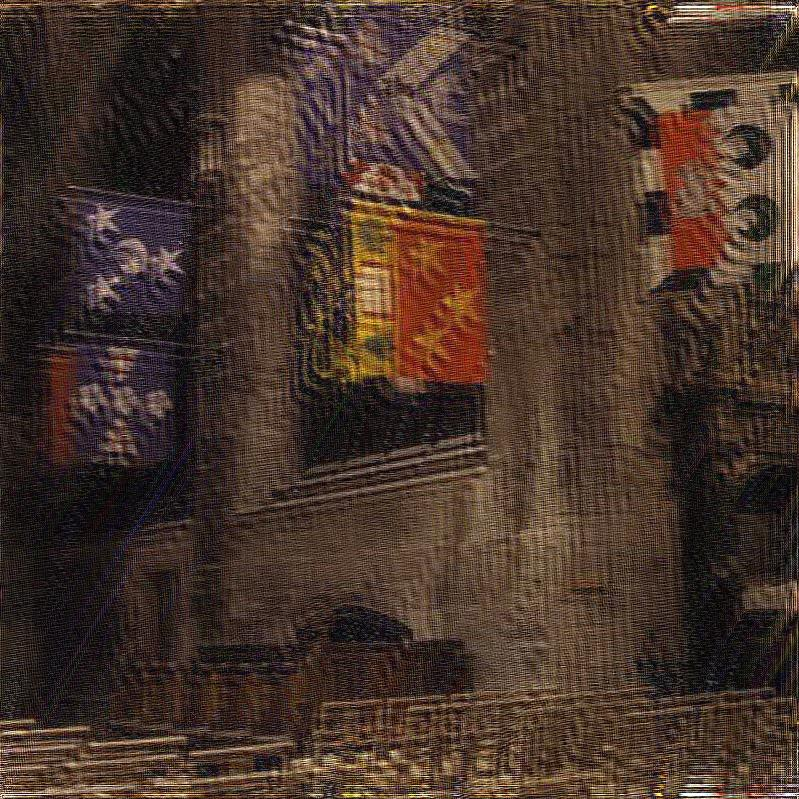
\includegraphics[width=8.5cm,height=0.20\textheight ]{Images/inv1_1.jpg}}
%  \vspace{2.0cm}
  \centerline{Test image after performing Inverse Filtering}\medskip
  PSNR:17.920233880580266 dB
  SSIM:0.008234314887168165
\end{minipage}
%
\end{figure}


\subsection{Radial Inverse Filtering}
\subsubsection{gamma = 150}
\begin{figure}[!htbp]

\begin{minipage}[!b]{1.0\linewidth}
  \centering
  \centerline{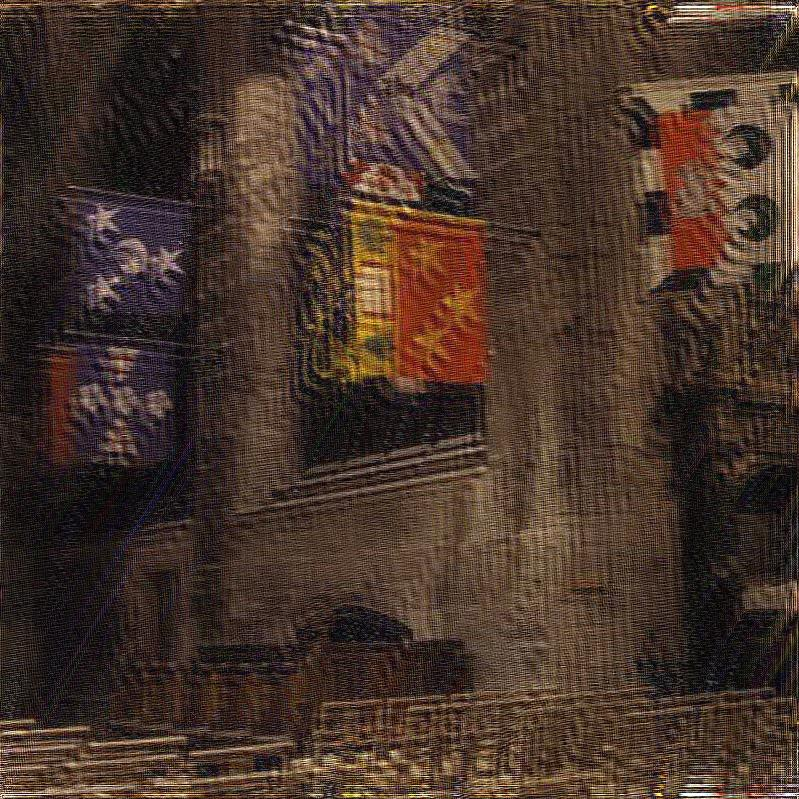
\includegraphics[width=8.5cm,height=0.350\textheight ]{Images/radial_150_1_1.jpg}}
%  \vspace{2.0cm}
  \centerline{Test image after performing Radial inverse filtering}\medskip
  PSNR:17.920233880580266 dB
  SSIM:0.008234314887168165
\end{minipage}
%
\end{figure}

\subsection[!htbp]{Weiner Filtering}

\begin{figure}[!htbp]

\begin{minipage}[!b]{1.0\linewidth}
  \centering
  \centerline{\includegraphics[width=8.5cm,height=0.350\textheight]{Images/weiner_01_1_1.jpg}}
%  \vspace{2.0cm}
  \centerline{Test image after Weiner Filtering with k = 0.1}\medskip
   PSNR:23.148784387462406 dB
  SSIM:0.12899297868054202
\end{minipage}
%
\end{figure}

\begin{figure}[!htbp]

\begin{minipage}[!b]{1.0\linewidth}
  \centering
  \centerline{
\includegraphics[width=8.5cm,height=0.350\textheight]{Images/weiner_5_1_1.jpg}}
%  \vspace{2.0cm}
  \centerline{Test image after Weiner Filtering with k = 5}\medskip
   PSNR:13.556953153524585 dB
  SSIM:0.014628983425784947
\end{minipage}
%
\end{figure}

\begin{figure}[!htbp]

\begin{minipage}[!b]{1.0\linewidth}
  \centering
  \centerline{
\includegraphics[width=8.5cm,height=0.350\textheight]{Images/weiner_8_1_1.jpg}}
%  \vspace{2.0cm}
  \centerline{Test image after Weiner Filtering with k = 8}\medskip
   PSNR:13.038407792002904 dB
  SSIM:0.006734134067439941
\end{minipage}
%
\end{figure}


\begin{figure}[!htbp]

\begin{minipage}[!b]{1.0\linewidth}
  \centering
  \centerline{
\includegraphics[width=8.5cm,height=0.350\textheight]{Images/weiner_15_1_1.jpg}}
%  \vspace{2.0cm}
  \centerline{Test image after Weiner Filtering with k = 15}\medskip
   PSNR:12.611057048090903 dB
  SSIM:0.0023642272982815336
\end{minipage}
%
\end{figure}



\subsection[!htbp]{Constrained LS Filtering}

\begin{figure}[!htbp]

\begin{minipage}[!b]{1.0\linewidth}
  \centering
  \centerline{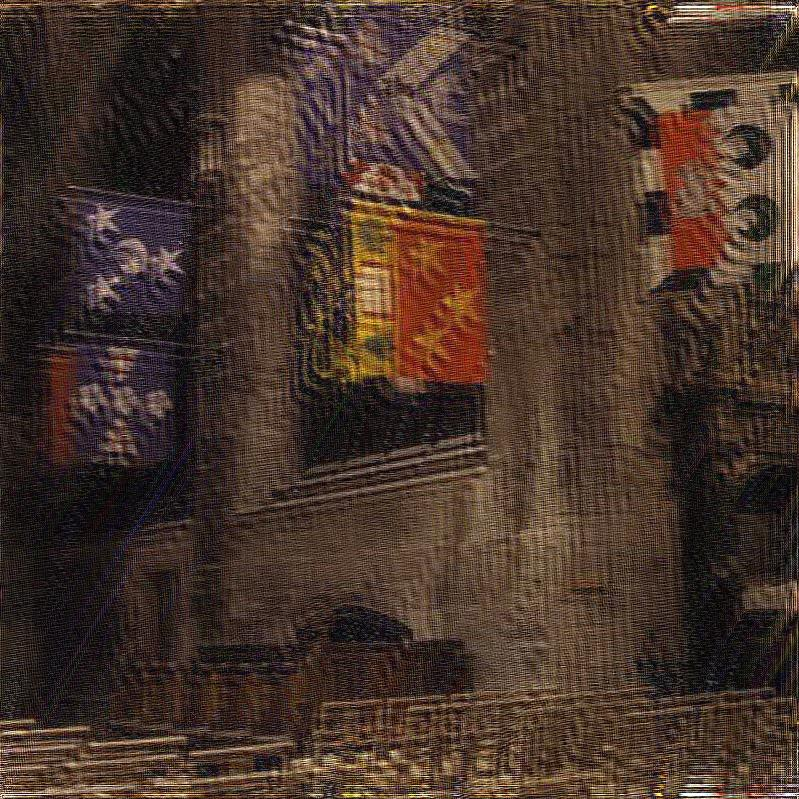
\includegraphics[width=8.5cm,height=0.20\textheight]{Images/LS_0_1_1.jpg}}
%  \vspace{2.0cm}
  \centerline{Image after applying LS filtering with gamma = 0}\medskip
  PSNR:17.920233880580266 dB
  SSIM:0.008234314887168165
\end{minipage}
%
\end{figure}

\begin{figure}[!htbp]

\begin{minipage}[!b]{1.0\linewidth}
  \centering
  \centerline{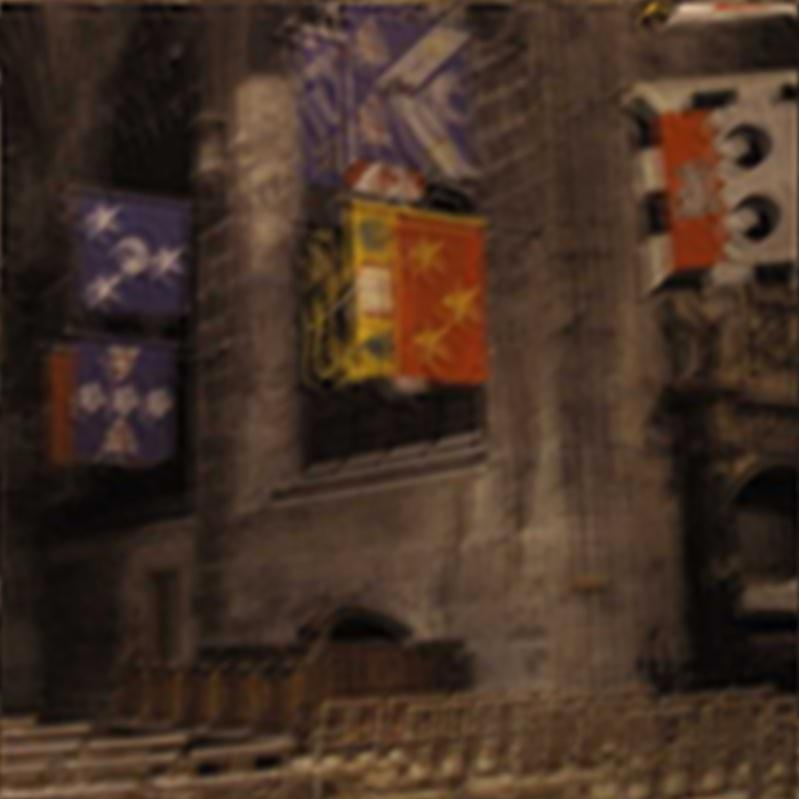
\includegraphics[width=8.5cm,height=0.20\textheight]{Images/LS_5_1_1.jpg}}
%  \vspace{2.0cm}
  \centerline{Image after applying LS filtering with gamma = 5}\medskip
  PSNR:24.42661193863731 dB
  SSIM:00.19684344630868653
\end{minipage}
%
\end{figure}

\begin{figure}[!htbp]

\begin{minipage}[!b]{1.0\linewidth}
  \centering
  \centerline{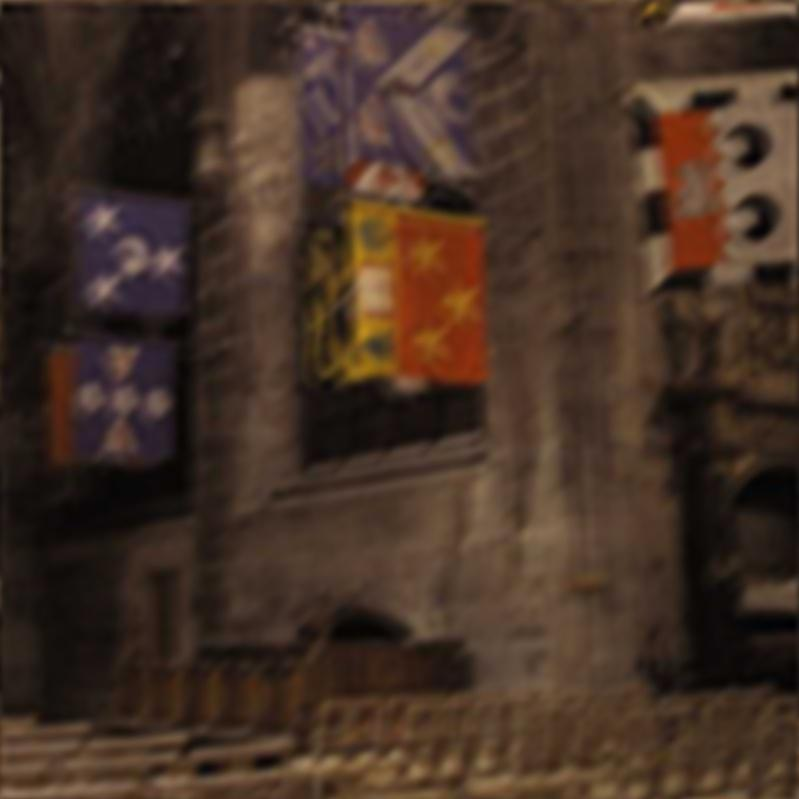
\includegraphics[width=8.5cm,height=0.20\textheight]{Images/LS_15_1_1.jpg}}
%  \vspace{2.0cm}
  \centerline{Image after applying LS filtering with gamma = 15}\medskip
  PSNR:24.43738047045613 dB
  SSIM:0.18830657461332967
\end{minipage}
%
\end{figure}

\begin{figure}[!htbp]

\begin{minipage}[!b]{1.0\linewidth}
  \centering
  \centerline{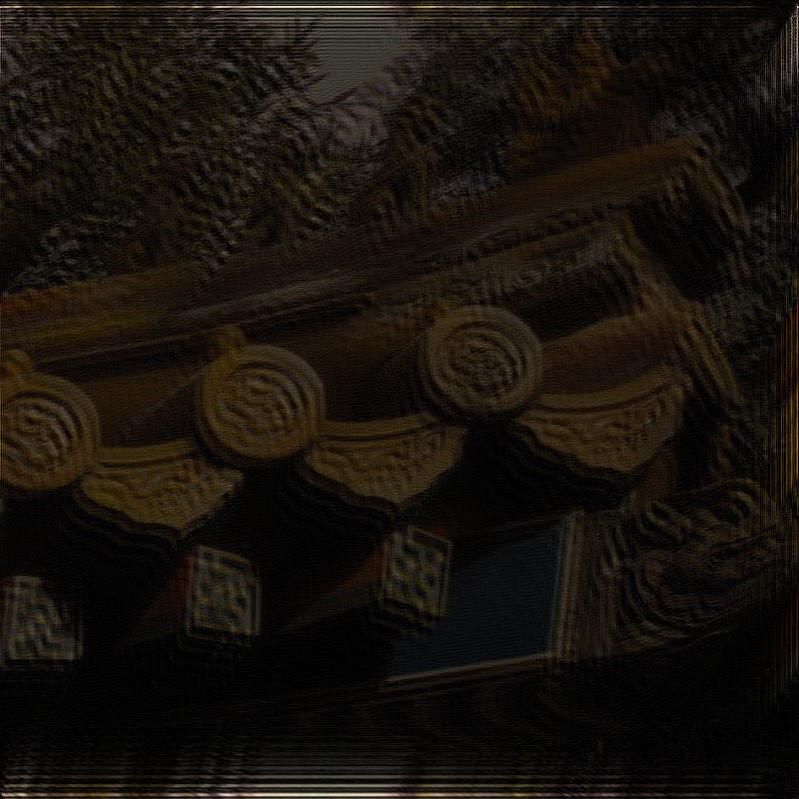
\includegraphics[width=8.5cm,height=0.20\textheight]{Images/LS_25_4_1.jpg}}
%  \vspace{2.0cm}
  \centerline{Image after applying LS filtering with gamma = 30}\medskip
  PSNR:24.38289276706215 dB
  SSIM:0.17594902052330422
\end{minipage}
%
\end{figure}
\subsection[!htbp]{Own Image}

\begin{figure}[!htbp]

\begin{minipage}[!b]{1.0\linewidth}
  \centering
  \centerline{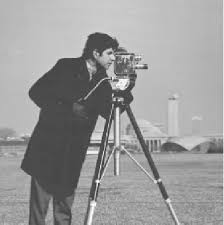
\includegraphics[width=8.5cm,height=0.20\textheight]{Images/test.jpeg}}
%  \vspace{2.0cm}
  \centerline{Degraded Image}\medskip

\end{minipage}
%
\end{figure}

\begin{figure}[!htbp]

\begin{minipage}[!b]{1.0\linewidth}
  \centering
  \centerline{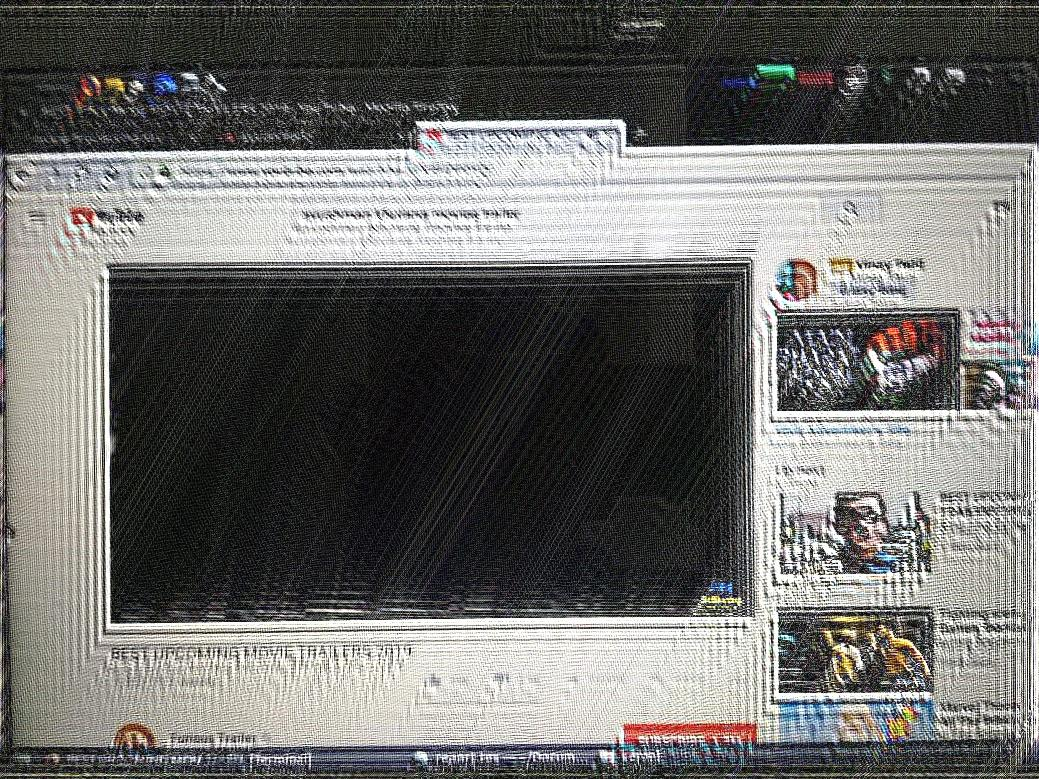
\includegraphics[width=8.5cm,height=0.20\textheight]{Images/test_inv.jpg}}
%  \vspace{2.0cm}
  \centerline{Image after applying Inverse filtering }\medskip

\end{minipage}
%
\end{figure}
\begin{figure}[!htbp]

\begin{minipage}[!b]{1.0\linewidth}
  \centering
  \centerline{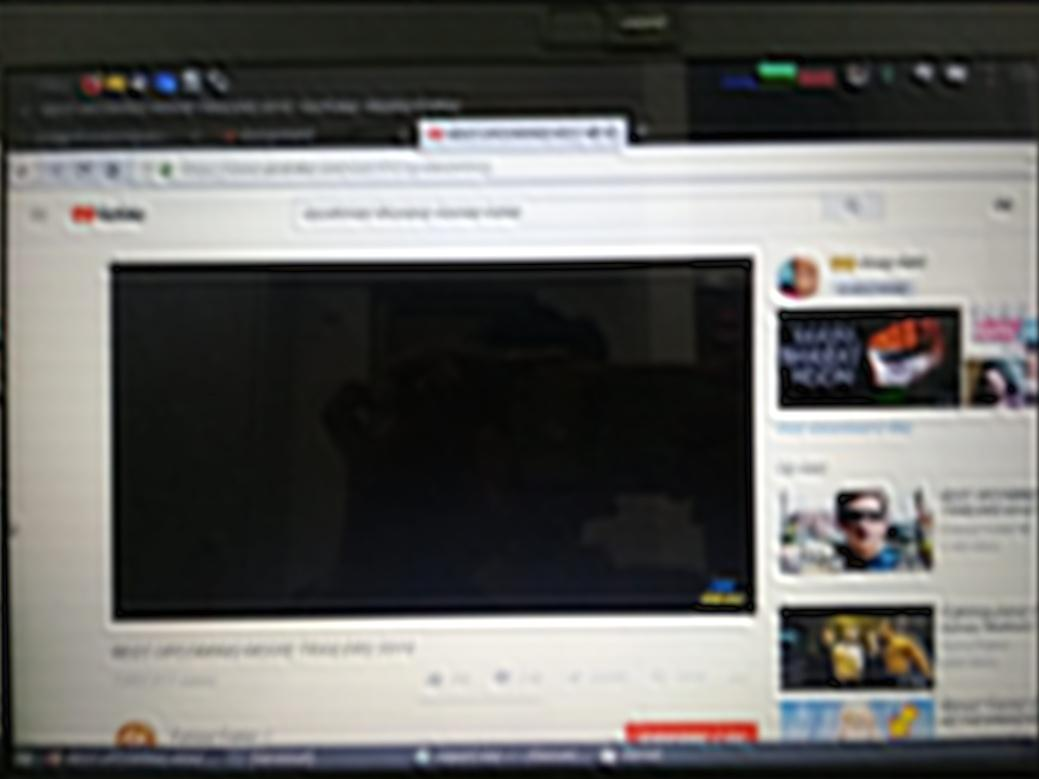
\includegraphics[width=8.5cm,height=0.20\textheight]{Images/test_ls_10.jpg}}
%  \vspace{2.0cm}
  \centerline{Image after applying LS filtering  with gamma = 10}\medskip

\end{minipage}
\end{figure}
\begin{figure}[!htbp]

\begin{minipage}[!b]{1.0\linewidth}
  \centering
  \centerline{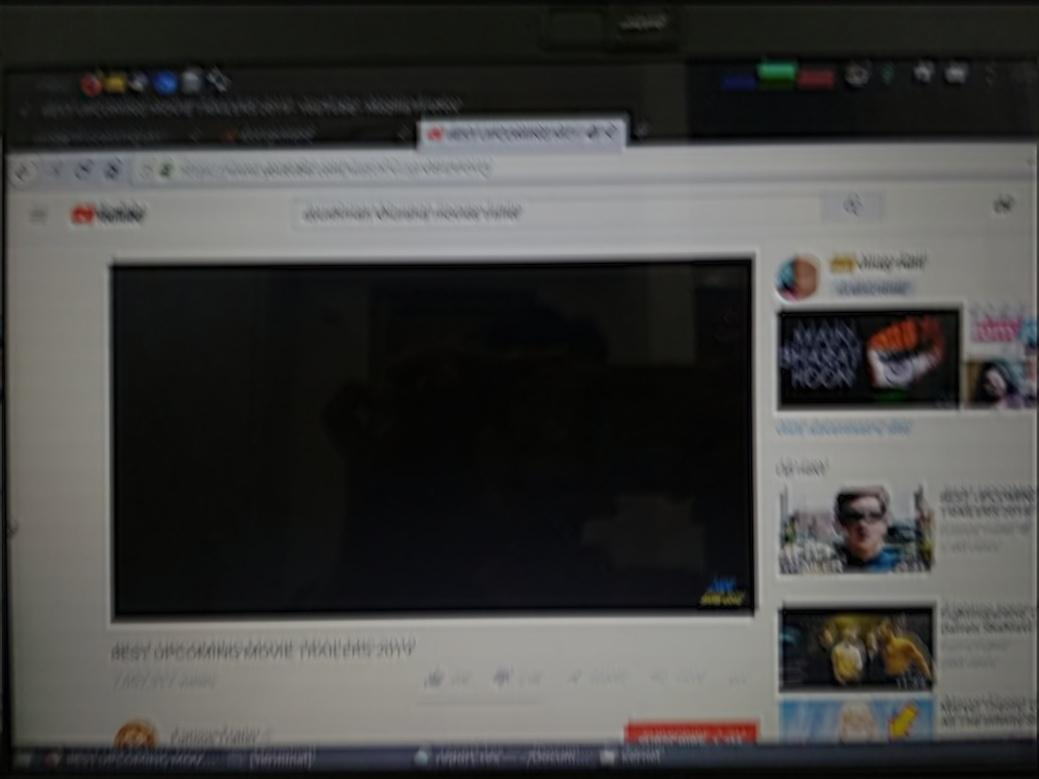
\includegraphics[width=8.5cm,height=0.20\textheight]{Images/test_wei_05.jpg}}
%  \vspace{2.0cm}
  \centerline{Image after applying Weiner filtering  with k = 0.5}\medskip

\end{minipage}
%
\end{figure}
\onecolumn
\section{Image 1 and kernel  1}
\begin{tabular}{|l|c|r|p{5cm} }
\hline
    Technique & PSNR(dB) & SSIM\\
    \hline
    Inverse Filtering & 17.920233880580266 & 0.008234314887168165\\
    \hline
    Radial Filtering & 17.920233880580266 & 0.008234314887168165\\
    \hline
    WEiner Filtering(k=0.1) & 23.148784387462406 & 0.12899297868054202\\
    \hline
    WEiner Filtering(k=5) & 13.556953153524585 & 0.014628983425784947\\
    \hline
    WEiner Filtering(k=8) & 13.038407792002904 & 0.006734134067439941\\
    \hline
    WEiner Filtering(k=15) & 12.611057048090903 & 0.0023642272982815336\\
    \hline
    LS Filtering(gamma = 0) & 17.920233880580266 & 0.008234314887168165\\
    \hline
    LS Filtering(gamma = 5 ) & 24.42661193863731 & 0.19684344630868653\\
    \hline
    LS Filtering(gamma = 15) & 24.43738047045613 &  0.18830657461332967\\
    \hline
    LS Filtering(gamma = 30 ) & 24.38289276706215 & 0.17594902052330422\\
    \hline
\end{tabular}
\section{Image 2 and kernel 2}
\begin{tabular}{|l|c|r|p{8cm} }
    \hline
    Technique & PSNR(dB) & SSIM\\
    \hline
    Inverse Filtering & 15.743600177961191 & 0.01806763382100661\\
    \hline
    Radial Filtering & 15.743600177961191 & 0.01806763382100661\\
    \hline
    WEiner Filtering(k=0.1) & 17.870996924435516 &  0.11471044241070671\\
    \hline
    WEiner Filtering(k=5) & 9.92043654165898 & 0.026220985543765552\\
    \hline
    WEiner Filtering(k=8) & 9.403203138009308 & 0.013683632943321195\\
    \hline
    WEiner Filtering(k=15) & 8.970344208679567 & 0.0054784068913342225\\
    \hline
    LS Filtering(gamma = 0) & 15.743600177961191 & 0.01806763382100661\\
    \hline
    LS Filtering(gamma = 5 ) & 18.499401965077773 & 0.17800703206835747\\
    \hline
    LS Filtering(gamma = 15) &18.862352697811325 &  0.1969149651622446\\
    \hline
    LS Filtering(gamma = 30 ) & 19.048974999571342 & 0.2013364186005355\\
    \hline
 \end{tabular}

\section{Image 3 and kernel 3}
\begin{tabular}{|l|c|r|}
    \hline
    Technique & PSNR(dB) & SSIM\\
    \hline
    Inverse Filtering & 21.20097119935902 & 0.007630150027224443\\
    \hline
    Radial Filtering & 21.20097119935902 & 0.007630150027224443\\
    \hline
    WEiner Filtering(k=0.1) & 21.338794848945035 &  0.031498087762106323\\
    \hline
    WEiner Filtering(k=5) & 10.872693095819962 & 0.011393571537853303\\
    \hline
    WEiner Filtering(k=8) & 10.335695115933085 & 0.009885694513261946\\
    \hline
    WEiner Filtering(k=15) & 9.894650159302431 & 0.002362223152195035\\
    \hline
    LS Filtering(gamma = 0) & 21.20097119935902 & 0.007630150027224443\\
    \hline
    LS Filtering(gamma = 5 ) & 22.456208024404198 &  0.03928754782333967\\
    \hline
    LS Filtering(gamma = 15) &22.769949599027072 &  0.06380004263981759\\
    \hline
    LS Filtering(gamma = 30 ) & 22.995828804296377 & 0.08294978860243511\\
    \hline
\end{tabular}
\section{Image 4 and blur kernel 4}
\begin{tabular}{|l|c|r|p{8cm}}
    \hline
    Technique & PSNR(dB) & SSIM\\
    \hline
    Inverse Filtering & 11.624179804769792 & 0.01806763382100661\\
    \hline
    Radial Filtering & 11.624179804769792 &  0.012311038805806343\\
    \hline
    WEiner Filtering(k=0.1) & 17.393370370384392 &  0.03811339259355565\\
    \hline
    WEiner Filtering(k=5) & 10.30338149892981 & 0.018064667816945604\\
    \hline
    WEiner Filtering(k=8) & 9.805246795009085 & 0.014313951901248873\\
    \hline
    WEiner Filtering(k=15) & 9.379381457812695 & 0..008265350751804708\\
    \hline
    LS Filtering(gamma = 0) & 11.624179804769792 & 0.012311038805806343\\
    \hline
    LS Filtering(gamma = 5 ) & 17.620551846304174 & 0.05629157888061678\\
    \hline
    LS Filtering(gamma = 15) &17.834248734468147 &  0.06413095520355722\\
    \hline
    LS Filtering(gamma = 30 ) & 18.003170165298194 & 0.07069987527622389\\
    \hline
\end{tabular}

\section{Discussion and Conclusion}
Entire Implementation is carried out under the assumption that the degraded images obtained are the result of convolution of the spatially invariant kernel  i.e., image is uniformly blurred by the same kernel. But the images taken are not spatially invariant. So the restored images are not likely to be as good as the ground truth, but the performance of several image restoration techniques can be studied.
\\ Inverse Filtering performs better only when there is no Noise or low Noise and also when the degradation is a result of the spatially invariant kernel. It is highly unsuitable for restoration in other cases.
\\ Radial Filtering is same as Inverse Filtering Except that it is passed through a Low pass filter after the Inverse Filtering. So it performs better than inverse filtering if the noise is low and kernel is spatially invariant. But in other cases it too fails miserably
\\Weiner Filtering is better that Radial and inverse Filters because it takes into account the noise distributed across the image and tries to preserve it so that the noise is not amplified. In this tool approximation of Weiner Filter is used by getting the ratio from the user which may cause performance loss. By looking at the tables above we can see that as the k value increases the Filtering becomes worse. So Weiner filtering gives best results when K is low (k< 1 ).
\\LS filtering also a good restoration technique. As the Implementation in this tool is a loose approximation of the actual filtering technique it may not give best result. The the gamma value is taken by the user but in actual technique it found in a iterative process and the optimum gamma would give good results. Also looking at the table one can say that as the gamma value increases the PSNR and SSIM increase. LS filtering works well for higher value of gamma but if these metircs are not taken into account and a subjective analysis of the output is done we can observe that the restored image is getting more and more blurred as the gamma is increased.
\\An image which is taken from my mobile is assumed to be degraded by the kernel 1. I tried to restore it by applying several techniques. Inverse filter and radial filter did not give satisfying results this might be because of the fact that the noise is not low and also the kernel is not spatially invariant. Weiner worked to some extent but it could not give exact restored image as the ground truth does not exist for this image it is difficult to say how good the restoration was. LS filtering gave the best results of all but as the gamma is increased more of blurring is happening.
\subsubsection{Learning}
Image restoration is not an exact maths as there are several factors which effect the performance of an restoration technique. The Techniques implemented here are functional under a lot of constrains . Machine Learning will be of great use because if the kernel and noise are estimated properly restoration is easy.
\section{Git Hub Link}
    \hyperref[https://github.com/M-ark17/Image-processing/tree/master/Assignment2]{''https://github.com/M-ark17/Image-processing/tree/master/Assignment2''}
\label{sec:ref}



% References should be produced using the bibtex program from suitable
% BiBTeX files (here: strings, refs, manuals). The IEEEbib.bst bibliography
% style file from IEEE produces unsorted bibliography list.
% -------------------------------------------------------------------------
% \bibliographystyle{IEEEbib}
\section{REFERENCES}
\begin{description}
    \item[$\cdot$ FFT] \hyperref[https://stackoverflow.com/questions/19739503/dft-matrix-in-python]{''https://stackoverflow.com/questions/19739503/dft-matrix-in-python''}
    \item[$\cdot$ padding] \hyperref[https://docs.scipy.org/doc/numpy/reference/generated/numpy.pad.html]{''https://docs.scipy.org/doc/numpy/reference/generated/numpy.pad.html''}
    \item[$\cdot$ Metrics] \hyperref[https://www.pyimagesearch.com/2017/06/19/image-difference-with-opencv-and-python/]{''https://www.pyimagesearch.com/2017/06/19/image-difference-with-opencv-and-python/''}
    \item[$\cdot$ Data Types] \hyperref[https://docs.scipy.org/doc/numpy-1.13.0/reference/arrays.dtypes.html]{''https://docs.scipy.org/doc/numpy-1.13.0/reference/arrays.dtypes.html''}
    \item[$\cdot$ MSE] \hyperref[https://stackoverflow.com/questions/20271479/what-does-it-mean-to-get-the-mse-mean-error-squared-for-2-images]{''https://stackoverflow.com/questions/20271479/what-does-it-mean-to-get-the-mse-mean-error-squared-for-2-images''}
    \item[$\cdot$ SSIM] \hyperref[http://scikit-image.org/docs/dev/api/skimage.measure.html]{''http://scikit-image.org/docs/dev/api/skimage.measure.html''}
    \item[$\cdot$ AND operator] \hyperref[https://stackoverflow.com/questions/609972/how-to-use-boolean-and-in-python ]{''https://stackoverflow.com/questions/609972/how-to-use-boolean-and-in-python ''}
    \item[$\cdot$ Numpy product of all elements] \hyperref[https://docs.scipy.org/doc/numpy-1.15.0/reference/generated/numpy.prod.html]{''https://docs.scipy.org/doc/numpy-1.15.0/reference/generated/numpy.prod.html''}
    \item[$\cdot$ PSNR] \hyperref[https://en.wikipedia.org/wiki/Peak_signal-to-noise_ratio ]{''https://en.wikipedia.org/wiki/Peak_signal-to-noise_ratio ''}

\end{description}
% \bibliography{strings,refs}
\onecolumn
\section{APPENDIX}
\subsection{Code using inbuilt FFT and IFFT functions }
\lstinputlisting[language=Python]{assignment2_1.py}
\subsection{Code  without using inbuilt FFT and IFFT functions }
\lstinputlisting[language=Python]{assignment2.py}
\end{document}
